\documentclass[10pt,a4paper]{amsart}
\usepackage[margin=19mm]{geometry}
\usepackage{amsmath,amssymb,mathtools}
\usepackage[scr=rsfs,cal=euler]{mathalfa}
\usepackage{xfrac}
\usepackage[unicode,hidelinks,bookmarks=false]{hyperref}
\newcommand{\ie}{i.e.\ }
\newcommand{\cf}{cf.\ }
\newcommand{\resp}{respectively\ }
\newcommand{\Subsection}{\subsection}
\providecommand{\nobreakdash}{\nobreak\hbox{-}}
\setlength{\emergencystretch}{2em}
\multlinegap0pt
\usepackage{tikz}
\usepackage{amssymb}
\usepackage{xcolor}
\usepackage{stackengine}
\newtheorem{proposition}{Proposition}
\title{\textbf{Ramanujan subshifts}}
\author{Ievgen Bondarenko, Rostislav Grigorchuk, Alina Vdovina}
\date{Source: arXiv:2602.22356v1 (CC BY 4.0)}
\begin{document}
\maketitle

\noindent\emph{Source and licence.} \textbf{Ramanujan subshifts}. Version arXiv:2602.22356v1 (CC BY 4.0), distributed by arXiv under the Creative Commons Attribution 4.0 International licence, http://creativecommons.org/licenses/by/4.0/, as recorded in the arXiv licence metadata for this exact version and shown on the abstract page https://arxiv.org/abs/2602.22356v1. Full licence notice: \texttt{licenses/arxiv-2602.22356-CC-BY-4.0.txt}.\par\smallskip

\noindent\textit{Editorial scope.} Counted unit: the article's proposition prop:ext\_matrix\_subshift\_is\_regular (source0.tex lines 815--835). The article's complete original proof of it is delivered with it (source0.tex lines 836--884, one \texttt{proof} environment of 49 lines). No mathematics is written, repaired or re-derived: the statement and the proof are the article's own lines, in the article's own notation, and no retained line is substituted or re-flowed.  No further source-local context is needed: every cross-reference of every retained line resolves inside the two delivered spans.  Nothing was omitted from any retained span, so the package carries no omission record.  No retained line contains a citation, so the wrapper carries no bibliography and no bibliography entry.  The retained lines contain the article's own diagram code, which the wrapper typesets with the standard tikz packages; no image file is delivered and the package declares no asset dependency.  Editorial formatting only, in addition: an AMS \texttt{amsart} preamble that restates the article's own declarations and macros used by the retained lines, namely the environments \texttt{proposition} on separate counters, together with the standard packages those lines need.  The retained environments print in this document as Proposition 1 in order of appearance, whereas the article prints the same items with the numbering of its own full document.  The complete native source of the article as distributed in the arXiv e-print for this exact version is bundled unchanged as \texttt{sources/195325/source0.tex}.
\begin{proposition}\label{prop:ext_matrix_subshift_is_regular}
Let $X=X(A,B)$ be an extendable matrix subshift defined by $d$-regular transition matrices $A$ and $B$. The following conditions are equivalent:
\begin{enumerate}
  \item The subshift $X$ is $d$-regular.
  \item The matrices $AB$ and $AB^\top$ have entries in $\{0,1\}$. In particular, $AB = BA$ and $AB^\top = B^\top A$.
  \item The subshift $X$ is uniquely extendable: every admissible pair of transitions along adjacent edges of a $(2,2)$-shape can be uniquely completed to an admissible $(2,2)$-pattern.
  \item The horizontal and vertical transition graphs $H_n(X)$ and $V_n(X)$ form $d$-fold covering families under the natural projection maps from $(n+1)$-patterns to $n$-patterns.
\end{enumerate}
Under these equivalent conditions, the subshift \( X(A, B) \) is homeomorphic to the subspace
\[
D(A,B)=\{ (x_h,x_v)\in X_A\times X_B : x_h(0)=x_v(0)  \}
\]
of the direct product \( X_A \times X_B \), where \( X_A \) and \( X_B \) are the one-dimensional subshifts defined by the transition matrices \( A \) and \( B \), respectively. This homeomorphism is given by
\[
\varphi: X(A, B)\rightarrow X_A \times X_B,  \quad  x \mapsto (x_h, x_v),
\]
where
\[
x_h(n) = x(n, 0), \qquad x_v(n) = x(0, n), \qquad \text{for all } n \in \mathbb{Z}.
\]
\end{proposition}

\begin{proof}
Since the matrices $A$ and $B$ are consistent, unique extendability is equivalent to the matrices $AB$ and $AB^\top$ having entries in $\{0,1\}$.

Every horizontal (resp. vertical) transition has exactly $d$ compatible vertical (resp. horizontal) transitions, and by the extendability condition, each such pair can be completed to an admissible $(2,2)$-pattern. If the subshift $X$ is $d$-regular, any admissible $(2,1)$-pattern admits exactly $d$ admissible extensions to a $(2,2)$-pattern. This means that each corner extension must be unique.
Conversely, unique extendability together with the $d$-regularity of $A$ and $B$ implies that every rectangular pattern admits exactly $d$ admissible extensions in each direction. This follows by induction on the size of the pattern: at each step, once one of the $d$ possible transitions is chosen for a single symbol, the rest of the extension is uniquely determined.

Let us consider the graphs $V_n=V_n(X)$. The vertices of $V_n$ are admissible $(n,1)$-patterns, and the edges correspond to valid vertical transitions. Define the natural projection
\[
\pi_r: V_{n+1}\rightarrow V_n, \ \pi_r(i_1,i_2,\ldots,i_{n+1})=(i_1,i_2,\ldots,i_{n}),
\]
which removes the rightmost symbol of the pattern. This projection is well-defined and maps edges to edges:
\begin{center}
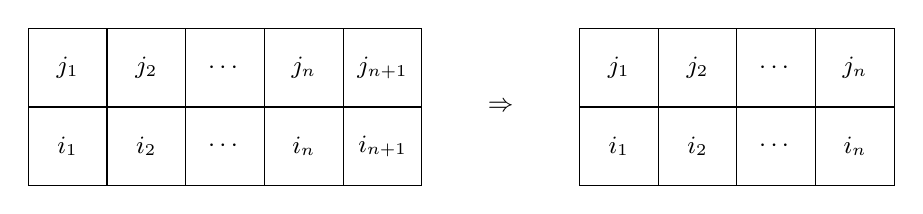
\begin{tikzpicture}[scale=1, every node/.style={font=\small}]
\foreach \x in {0,...,4} {
    \draw (\x,0) rectangle ++(1,1); % bottom row
    \draw (\x,1) rectangle ++(1,1); % top row
}
\foreach \x in {0,1} {
    \node at (\x+0.5,0.5) {$i_{\the\numexpr\x+1}$}; % bottom
    \node at (\x+0.5,1.5) {$j_{\the\numexpr\x+1}$}; % top
}
\node at (3+0.5,0.5) {$i_{n}$}; % bottom
\node at (3+0.5,1.5) {$j_{n}$}; % top
\node at (4+0.5,0.5) {$i_{n+1}$}; % bottom
\node at (4+0.5,1.5) {$j_{n+1}$}; % top
\node at (2.5,0.5) {$\cdots$};
\node at (2.5,1.5) {$\cdots$};

\node at (6,1) {$\Rightarrow$};

\foreach \x in {7,...,10} {
    \draw (\x,0) rectangle ++(1,1); % bottom row
    \draw (\x,1) rectangle ++(1,1); % top row
}

\node at (7+0.5,0.5) {$i_{1}$}; % bottom
\node at (7+0.5,1.5) {$j_{1}$}; % top
\node at (8+0.5,0.5) {$i_{2}$}; % bottom
\node at (8+0.5,1.5) {$j_{2}$}; % top
\node at (7+3+0.5,0.5) {$i_{n}$}; % bottom
\node at (7+3+0.5,1.5) {$j_{n}$}; % top
\node at (7+2.5,0.5) {$\cdots$};
\node at (7+2.5,1.5) {$\cdots$};
\end{tikzpicture}
\end{center}
The projection $\pi_r$ induces a bijection on the set of directed edges passing from a vertex if and only if the unique extendability condition holds for the upper-right corner (here $j_{n+1}$ should be uniquely defined by $i_{n+1}$ and $j_n$). Similarly, $\pi_r$ is bijective on incoming edges to a vertex if the unique extendability condition holds for the lower-right corner. Analogously, the projection $\pi_l$, which removes the leftmost symbol, is a covering map when unique extendability holds for the upper-left and lower-left corners.  The same characterization applies to the graphs $H_n(X)$.

Finally, the unique extendability condition ensures that every admissible configuration is uniquely determined by its horizontal and vertical traces, i.e., by the sequences of admissible horizontal and vertical transitions along the coordinate axes. Therefore, the map $\varphi$ is bijective and maps rectangular cylinder sets to products of cylinder sets.
\end{proof}

\end{document}
